\subsection{Phases et sénarios de vol}
\label{subsec:phases_scenarios_vol}

\subsubsection{Phases de vol}
\label{subsec:phases_vol}

Le vol de la fusée SP-02 se déroule selon six phases successives représentées dans la figure suivante. Ce découpage permet
d’identifier clairement les séquences critiques du lanceur.

\begin{figure}[h!]
\centering
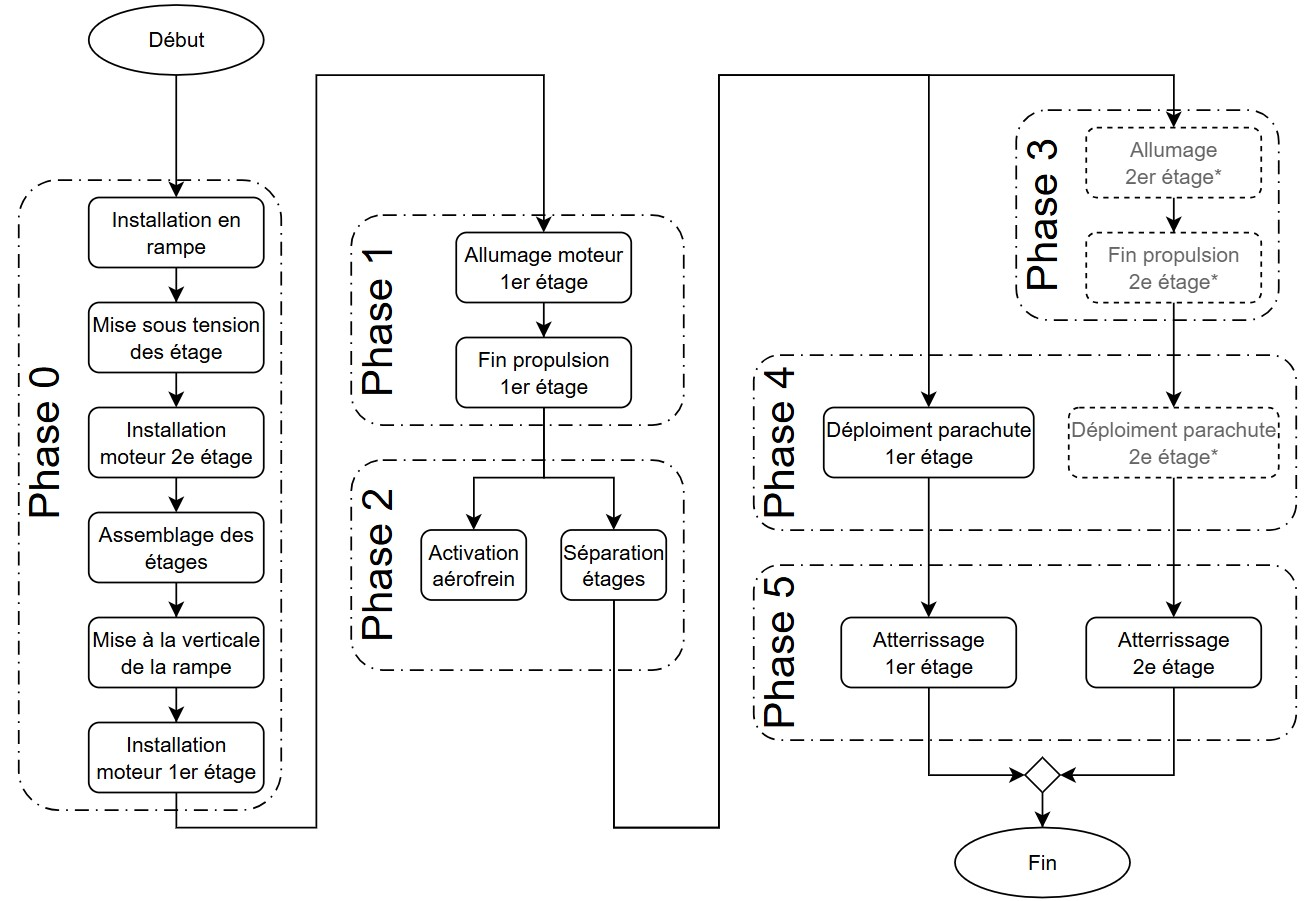
\includegraphics[width=\textwidth]{figures/Phase_de_vol.jpg}
\caption{Diagramme des phases nominales de vol depuis SP-02}
\end{figure}

Les éléments marqué d'un " * " sont des éléments optionelles.

\subsubsubsection*{Phase 0 — Préparation et mise en condition du système}
\begin{itemize}
    \item \textbf{État initial} : Le lanceur est en configuration d’intégration au sol : les deux étages sont séparés, non armés, et
    aucun sous-système pyrotechnique ou avionique n’est actif.
    \item \textbf{Objectif fonctionnel} : Placer le système dans un état prêt au lancement, en assurant que :
    \begin{itemize}
        \item les étages sont correctement assemblés,
        \item les systèmes avioniques sont initialisés et opérationnels,
        \item les sécurités pyrotechniques sont actives,
        \item les conditions mécaniques et géométriques sont conformes (verticalité, contrainte au rail).
    \end{itemize}
    \item \textbf{Règles du \acrshort{CDC} ASF2 concernées}
    \begin{itemize}
        \item MAF1-MAF8\cite[p. ~68-70]{CDC_BiEtage} : système d'allumage compatible et sécurisé.
        \item INF1-INF3\cite[p. ~73-75]{CDC_BiEtage} : conformité de l'inflammateur et des connectiques.
        \item SPYTC1-SPYTC4\cite[p. ~76-77]{CDC_BiEtage} : sécurité pyrotechnique conforme aux spécifications.
        \item ORDRE1, ORDRE5\cite[p. ~78-80]{CDC_BiEtage} : logique d'armement et de commande découplé de l'inflammateur et sûr.
        \item FTP1-FTP4\cite[p. ~84-86]{CDC_BiEtage} : système de démarrage de la chronométrie prêt et conforme.
    \end{itemize}
\newpage
    \item \textbf{État final attendu} : La fusée est mécaniquement stable, correctement armée mais sécurisée, prête à entrer en
    phase 1 :
    \begin{itemize}
        \item alimentation disponible mais protégée,
        \item ligne pyro sous shunt,
        \item avionique synchronisée,
        \item attitude et verticalité conformes.
        \item système mécaniquement stable et apte à supporter la propulsion du premier étage.
    \end{itemize}
\end{itemize}

\subsubsubsection*{Phase 1 — Propulsion et ascension du premier étage}
\begin{itemize}
    \item \textbf{État initial} : La Fusée est armée, l'autorisation sol donnée, le moteur du 1er étage est au repos les capteurs et
    séquenceurs sont armés et prêts au lancement.
    \item \textbf{Objectif fonctionnel} : Assurer une ascension stable, sans perte de gabarit, jusqu’à l’altitude et la vitesse
    permettant une séparation sûre et effective des deux étages.
    \item \textbf{Règles du \acrshort{CDC} ASF2 concernées} :
    \begin{itemize}
        \item MAF1-MAF8\cite[p. ~68-70]{CDC_BiEtage} : L'accélération subie ne doit pas compromettre le système d'allumage.
        \item INF1-INF3\cite[p. ~73-75]{CDC_BiEtage} : L'accélération subie ne doit pas compromettre le fonctionnement de l'inflammateur.
        \item ORDRE2, ORDRE4\cite[p. ~78-80]{CDC_BiEtage} : mesure du temps depuis l’allumage du moteur du 1er étage.
        \item ATT1-ATT4\cite[p. ~81-83]{CDC_BiEtage} : L'accélération subie ne doit pas compromettre le système de vérification d’attitude du 2nd étage.
        \item FTP1-FTP4\cite[p. ~84-86]{CDC_BiEtage} : fenêtre temporelle de vol du 1er étage fonctionnelle.
        \item SEP1-SEP3\cite[p. ~87-88]{CDC_BiEtage} : L'accélération subie ne doit pas compromettre le système de détection de séparation.
    \end{itemize}
    \item \textbf{État final attendu} Le premier étage atteint sa fin de propulsion :
    \begin{itemize}
        \item stabilité assurée,
        \item vitesse suffisante,
        \item avionique en état de détecter la transition vers la séparation.
    \end{itemize}
\end{itemize}

\subsubsubsection*{Phase 2 — Séparation par aérofreinage}
\begin{itemize}
    \item \textbf{État initial} : Les deux étages volent conjointement en balistique post-propulsion.
    \item \textbf{Objectif fonctionnel} : Obtenir une séparation passive, franche et symétrique, générée par un différentiel
    de traînée créé par l’ouverture d'aérofreins sur le premier étage.
    \item \textbf{Règles du \acrshort{CDC} ASF2 concernées} :
    \begin{itemize}
        \item ORDRE2, ORDRE4\cite[p. ~78-80]{CDC_BiEtage} : système de détection de la séparation fiable.
        \item SEP1, SEP2\cite[p. ~87-88]{CDC_BiEtage} : système de détection de la séparation fiable.
        \item SEP3\cite[p. ~87-88]{CDC_BiEtage} : ordre de séparation donné uniquement à la fin de propulsion du 1er étage.
    \end{itemize}
    \item \textbf{État final attendu} : Les deux étages sont nettement séparés et évoluent sur des trajectoires distinctes ; le
    2e étage se trouve dans un état compatible avec un éventuel allumage. Une confirmation fiable de séparation doit être
    établie par l’avionique des deux étages.
\end{itemize}

\subsubsubsection*{Phase 3 — Propulsion du second étage}
\begin{itemize}
    \item \textbf{État initial} : Le second étage est séparé, stabilisé et en attente de conditions d’autorisation d’allumage.
    \item \textbf{Objectif fonctionnel} : Allumer le moteur du 2e étage uniquement si les trois critères suivants sont
    satisfaits simultanément :
    \begin{enumerate}
        \item Séparation confirmée
        \item Attitude dans le domaine acceptable
        \item Fenêtre temporelle active
    \end{enumerate}
\newpage
    \item \textbf{Règles du \acrshort{CDC} ASF2 concernées} :
    \begin{itemize}
        \item MAF1-MAF8\cite[p. ~68-70]{CDC_BiEtage} : sécurités et alimentation de la ligne pyrotechnique.
        \item INF1-INF3\cite[p. ~73-75]{CDC_BiEtage} : compatibilité avec l’inflammateur.
        \item ORDRE1-ORDRE5\cite[p. ~78-80]{CDC_BiEtage} : logique d’autorisation/commande d’allumage.
        \item ATT1-ATT4\cite[p. ~81-83]{CDC_BiEtage} : vérification d’attitude avant allumage.
        \item FTP1-FTP4\cite[p. ~84-86]{CDC_BiEtage} : fenêtre temporelle d’allumage conforme.
    \end{itemize}
    \item \textbf{État final attendu} : Deux cas :
    \begin{itemize}
        \item Cas nominal : Allumage du moteur du 2e étage autorisé : montée propulsive stable.
        \item Cas sécurisé : Conditions non réunies : allumage définitivement interdit.
    \end{itemize}
    Dans tous les cas, la trajectoire doit rester dans le gabarit.
\end{itemize}

\vspace{-0.4cm}

\subsubsubsection*{Phase 4 — Ouverture des parachutes et descente des étages}
\vspace{-0.2cm}
\begin{itemize}
    \item \textbf{État initial} : Les deux étages sont séparés et en trajectoire balistique, le 2e étage a ou non allumé son moteur.
    \item \textbf{Objectif fonctionnel} : Assurer un retour sécurisé au sol via :
    \begin{itemize}
        \item une détection robuste de l’apogée,
        \item l’ouverture fiable de la trappe d’éjection,
        \item le déploiement du parachute.
    \end{itemize}
    \item \textbf{Règles du \acrshort{CDC} ASF2 concernées} : (pas de règle spécifique à cette phase décrite par la rubrique ASF
    du \acrshort{CDC})
    \item \textbf{État final attendu} : Là aussi pour chaque étage, deux cas sont possibles :
    \begin{itemize}
        \item Cas nominal : Apogée détectée, trappe éjectée, parachute déployé.
        \item Cas balistique : Echec du système de détection d’apogée ou d’éjection de trappe : chute libre contrôlée.
    \end{itemize}
    Dans les deux cas, les trajectoires de descente restent dans le gabarit de sécurité défini par le \acrshort{CDC}.
\end{itemize}

\vspace{-0.4cm}

\subsubsubsection*{Phase 5 — Atterrissage et récupération}
\vspace{-0.2cm}
\begin{itemize}
    \item \textbf{État initial} : Les deux étages descendent sous parachute ou en chute libre contrôlée.
    \item \textbf{Objectif fonctionnel} : Assurer un atterrissage en toute sécurité dans le gabarit défini, minimisant les
    risques pour les personnes, les biens et l’environnement.
    \item \textbf{Règles du \acrshort{CDC} ASF2 concernées} : (pas de règle spécifique à cette phase décrite par la rubrique ASF
    du \acrshort{CDC})
    \item \textbf{État final attendu} : Ici aussi, deux cas pour chaque étage définis par la phase précédente :
    \begin{itemize}
        \item Cas nominal : Atterrissage sous parachute dans le gabarit, étage intact.
        \item Cas balistique : Atterrissage en chute libre contrôlée dans le gabarit, étage détruit.
    \end{itemize}
    Dans les deux cas, l’atterrissage doit se faire sans risque pour les personnes, les biens et l’environnement.
\end{itemize}

% \newpage
\vspace{-0.4cm}

\subsubsection{Scénarios de vol}

Deux des évenement du vol influe particulièrement le profile de vol de la mission :

\hspace*{-\parindent}%
\begin{minipage}{0.6\textwidth}
    \begin{itemize}
        \item \textbf{Séparation} : Le système de séparation des deux étages de la fusée est considéré comme un système expérimental. Son bon foncionnement
        n'est donc pas un élément certain. Le non délpoiement de ce dernier correspond au scénario \texttt{SCE2}.
        \item \textbf{Allumage 2e étage} : L'allumage du moteur du deuxième étage est également un système expérimental. De plus, pour des raisons de
        sécurité, cet allumage ne doit être effectué que si la trajectoire courante respecte un certain gabarie. On distinguera alors deux sous-cas :
        \begin{itemize}
            \item La trajectoire ne respecte pas la plage de sécurité (scénario \texttt{SCE1.1})
            \item Le système d'allumage n'a pas fonctionné (scénario \texttt{SCE1.2})
        \end{itemize}
        Ces deux scénarios font partie du même scénario \texttt{SCE1} qui décrit le non allumage du moteur du deuxième étage.
    \end{itemize}
\end{minipage}
\hfill
\begin{minipage}{0.4\textwidth}
    \centering
    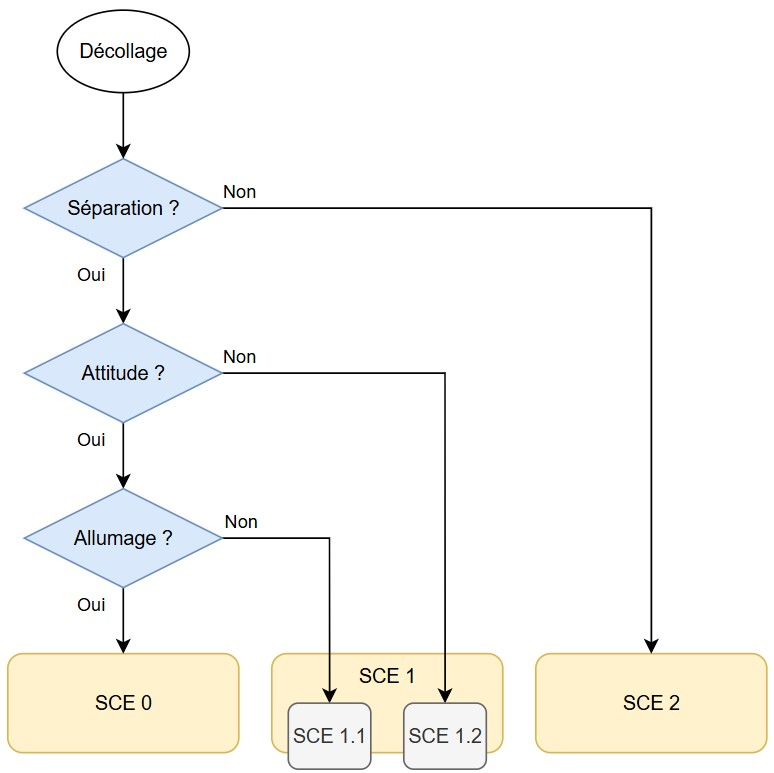
\includegraphics[width=\textwidth]{figures/SCE.jpg}
    \captionof{figure}{Différent scénarios}
    \label{fig:sces}
\end{minipage}

\newpage
